\documentclass{article}

% Language setting
% Replace `english' with e.g. `spanish' to change the document language
\usepackage[english]{babel}

% Set page size and margins
% Replace `letterpaper' with `a4paper' for UK/EU standard size
\usepackage[letterpaper,top=2cm,bottom=2cm,left=3cm,right=3cm,marginparwidth=1.75cm]{geometry}

% Useful packages
\usepackage{amsmath}
\usepackage{amssymb}
\usepackage{graphicx}
\usepackage[colorlinks=true, allcolors=blue]{hyperref}
\usepackage{braket} 
\title{Daily Note}
\author{You}


\begin{document}
	\maketitle
	
	\section{integration of green function in time with classical fft:}
	
	We want to perform the following integration:
	
	\begin{align}
		g^{c}(\tau) &= \int_a^b \frac{1}{2\pi} dE g^c(E)e^{-iE\tau}
	\end{align}
	
	\begin{align}
		g^{c}(E) &= \int d\tau g^c(\tau)e^{iE\tau}
	\end{align}
	
	First we discretize the energy of the whole finite energy $[a,b]$ domaine using N points:
	
	\begin{align}
		E_n &= E_0 + n\Delta E,\\
		E_0 &= a,\\
		\Delta_E &= \frac{b-a}{N}.
	\end{align}
	
	Then we rewrite our integral with Riemann sum:
	
	\begin{align}
		g^{c}(\tau) &= \frac{1}{2\pi} \sum_{n=0}^{N-1}  \Delta E g^c(E_n)e^{-iE_n\tau}.
	\end{align}
	
	We then do a similar discretization on the time $\tau$:
	
	\begin{align}
		\tau_m = m \Delta \tau.
	\end{align}
	
	We can rewrite our integration:
	
	\begin{align}
		g^{c}(\tau_m) &= \frac{\Delta E}{2\pi} \sum_{n=0}^{N-1}   g^c(E_n)e^{-i(E_0 + n\Delta E)m \Delta \tau},\\
		g^{c}(\tau_m) &= e^{-iE_0m \Delta \tau} \frac{\Delta E}{2\pi} \sum_{n=0}^{N-1} g^c(E_n)e^{-inm\Delta E \Delta \tau}.
	\end{align}
	
	The FFT (Fast Fourier Transform) is:
	
	\begin{align}
		X_m &= \sum_{n=0}^{N-1}x_ne^{-2\pi{}i\frac{n m}{N}}. % chktex 25
	\end{align}
	
	We identify:
	
	\begin{align}
		\Delta E \Delta \tau &= \frac{2\pi}{N}
	\end{align}
	
	Giving us the fft integration:
	
	\begin{align}
		g^{c}(\tau_m) &= e^{-iE_0m \Delta \tau} \frac{\Delta E}{2\pi} \sum_{n=0}^{N-1} g^c(E_n)e^{-\frac{i2\pi nm}{N}}
	\end{align}
	
	
	If we want to avoid border artifact, we can add padding to each side of our function. Finally we want to center the time to introduce the negative time correctly.
	
	\begin{align}
		\tau_m = \begin{cases} 
			\tau_m & \text{ positive time if } m<\frac{N}{2}, \\
			\tau_m & \text{negative time if } m>\frac{N}{2}
		\end{cases}
	\end{align}
	
	WARNING Due to Kwant convention, we can remove the factor 1/2pi:
	
	\begin{align}
		g^{c}(\tau_m) &= e^{-iE_0m \Delta \tau} \Delta E \sum_{n=0}^{N-1} g^c(E_n)e^{-\frac{i2\pi nm}{N}}
	\end{align}
	
	\section{mps:}
	
	\subsection{fft with qft:}
	We want to do all these operation in terms of mps. And we will use the full extend of tensor network by using the QFT (quantum fourier transform) that we construct as an mpo with the leg exposed like follow:
	\begin{eqnarray}
		t^{k:q} &=& t_k + 2t_{k+1} +\cdots + 2^{q-k} t_{q}, \\
		\omega^{k:q} &=& 2^{q-k} \omega_k + 2^{q-k-1}\omega_{k+1} +\cdots +  \omega_{q},
	\end{eqnarray}
	
	\begin{align}
		QFT(x,k) = y_k &= \frac{1}{\sqrt{N}}\sum_{j=0}^{N-1}x_j w_N^{-jk},\\
		w_n &= e^{\frac{2i\pi}{N}}.
	\end{align}
	
	We can thus map the FFT operation to a QFT like this:
	
	\begin{align}
		g^{c}(\tau_m) &= e^{-iE_0m \Delta \tau} \sqrt{N} \Delta E  \frac{1}{\sqrt{N}}\sum_{n=0}^{N-1} g^c(E_n)e^{-nm\frac{2i\pi}{N}}, \\
		g^{c}(\tau_m) &= e^{-iE_0m \Delta \tau} \sqrt{N} \Delta E  \frac{1}{\sqrt{N}}\sum_{n=0}^{N-1} g^c(E_n)w_N^{-nm}, \\
		g^{c}(\tau_m) &= e^{-iE_0m \Delta \tau}  \Delta E \sqrt{N} QFT(g^c(E),m)
	\end{align}
	
	\subsection{fft trapeze:}
	
	The FFT treats the sampled function as periodic. If the endpoint values $f(a)$ and $f(b)$ differ, the periodic extension has a jump and convergence can slow to $O(1/N)$.
	The fft grid by definition doesn't use the value in b. By using the trapeze quadrature on the summation and providing the additional value in b we should be able to have an error decreasing in 1/2N instead. 
	
	\begin{align}
		\forall E \in [a, b]: g^c(E)\\
		\tilde{g}^c(E_n) = 
		\begin{cases}
			\frac{1}{2} g^c(E_0) & n = 0 \\
			g^c(E_n) & 1 \leq n \leq N-1
		\end{cases}
	\end{align}
	
	\begin{align}
		g^{c}(\tau_m) &= e^{-iE_0m \Delta \tau}  \Delta E \left( \sqrt{N} QFT(\tilde{g}^c(E),m) + \frac{1}{2} g^c(b) \right)
	\end{align}
	\begin{figure}[ht]
		\centering
		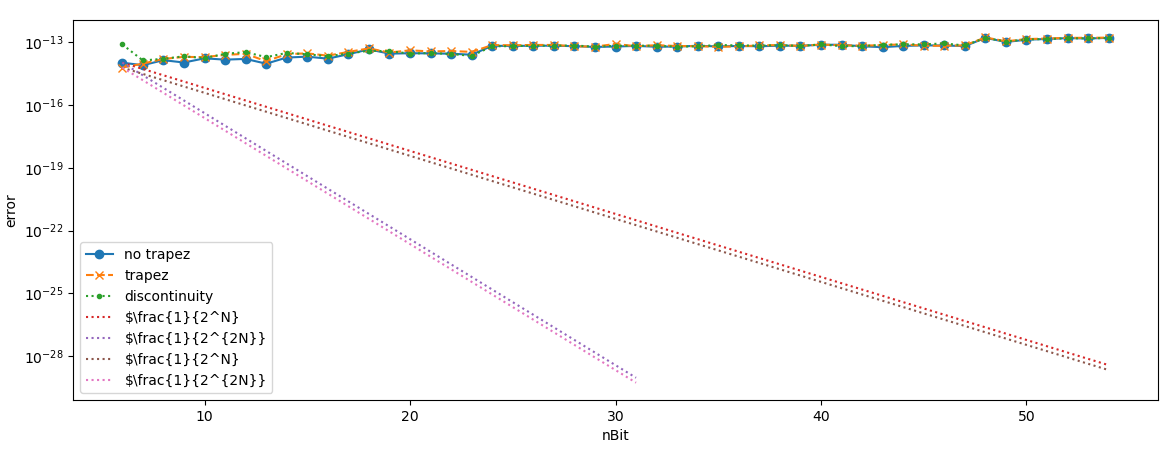
\includegraphics[width=0.8\textwidth]{figure/smoth_and_periodic_function.png}
		\caption{smoth and periodic function, exponential decrease rate of the error}
	\end{figure}
	
	
	\begin{figure}[ht]
		\centering
		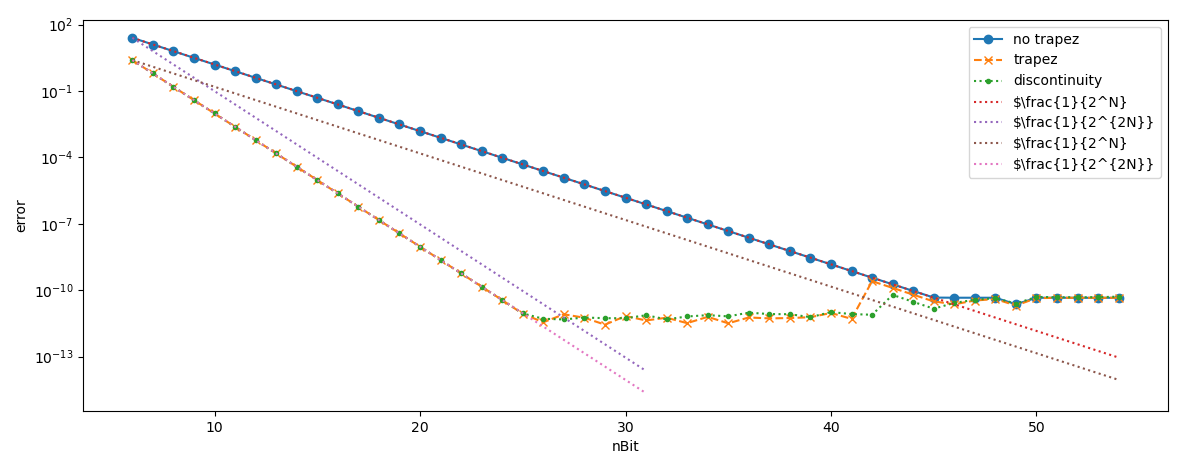
\includegraphics[width=0.8\textwidth]{figure/discontinuous_end_point.png}
		\caption{discontinuous end point case, 1/2N decrease rate where end points are fixed by trapez quadrature}
	\end{figure}
	
	\subsection{fft trapez discontinuity}
	
	We can also have 1/2N error scaling in the case of discontinuous interval by splitting the fft in halve at the exact position of the discontinuity.
	
	We have to respect two very strict condition:
	\begin{itemize}
		\item The discontinuity must fall exactly on grid point. Else we get 1/N error
		\item point where we split must be the first point of the next interval
	\end{itemize}
	
	\begin{figure}[ht]
		\centering
		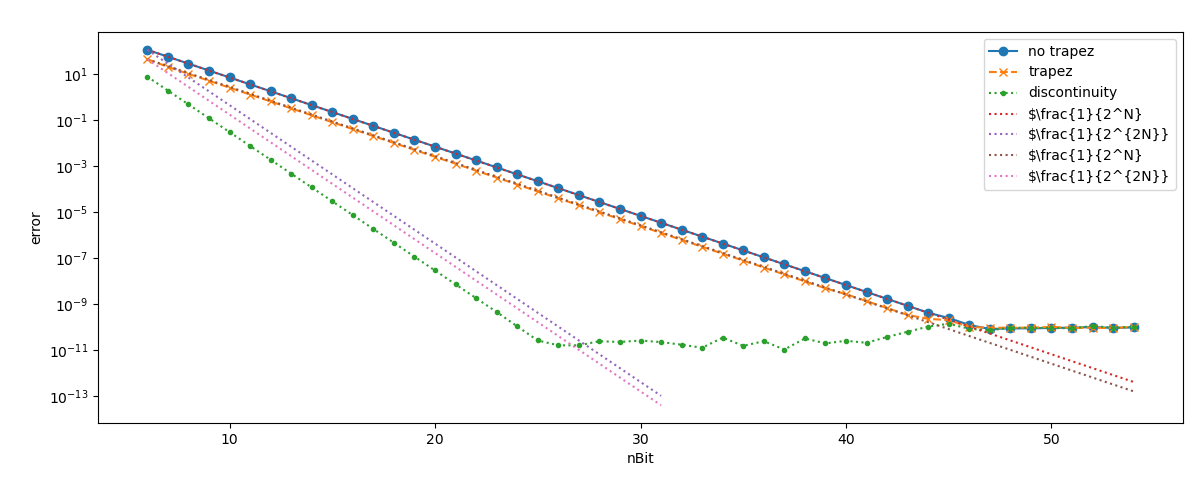
\includegraphics[width=0.8\textwidth]{figure/2_discontinuity_function_case.png}
		\caption{2 discontinuity function case, 1/2N decrease of the error where internal discontinuity are fixed with trapeze quadrature}
	\end{figure}
	
	\section{Remarque on fft}
	
	The convergence speed depend on the smoothness on the border of the interval. If the function is $C^k$ at the border of the interval, the convergence speed is $\frac{1}{kN}$.
	With the trapeze method, we are able to cancel out the error in $\frac{1}{N}$, leaving us with an error in $\frac{1}{2N}$.
	
	\section{update}

	\subsection{MPS/MPO form of the trapezoid FFT}
	
	Let $R$ be the number of bits, $N=2^R$, and write the energy index MSB-first as
	$n = \sum_{k=1}^{R} n_k 2^{R-k}$. We introduce
	
	\begin{itemize}
		\item $\ket{g_E}$: the MPS encoding $g^c(E_n)$,
		\item $\hat{W}$: the diagonal trapezoid MPO, $W_n = \tfrac12 \delta_{n,0} + (1-\delta_{n,0})$,
		\item $\ket{\delta_{N_0}}$: the single-point MPS at index $N_0$,
		\item $\ket{\mathbb{1}}$: the constant MPS,
		\item $\widehat{QFT}$: the QFT MPO, $\widehat{QFT}_{mn} = \tfrac{1}{\sqrt N} e^{-2i\pi nm/N}$,
		\item $\hat{P}$: the diagonal phase MPO $e^{-iE_0 \tau_m}$, with $\tau_m$ in two's complement.
	\end{itemize}
	
	With padding ($N = 2^p N_0$, so $b$ lies on the grid at index $N_0$):
	\begin{align}
		\ket{g_\tau} = \frac{\Delta E}{2\pi}\, \hat{P}\, \sqrt{N}\, \widehat{QFT}
		\left[ \hat{W}\ket{g_E} + \frac{g^c(b)}{2}\ket{\delta_{N_0}} \right].
	\end{align}
	
	Without padding ($N = N_0$, $b$ aliases onto index $0$):
	\begin{align}
		\ket{g_\tau} = \frac{\Delta E}{2\pi}\, \hat{P}
		\left[ \sqrt{N}\, \widehat{QFT}\, \hat{W}\ket{g_E} + \frac{g^c(b)}{2}\ket{\mathbb{1}} \right].
	\end{align}
	
	The second expression follows from the first: $\sqrt{N}\,\widehat{QFT}\ket{\delta_N}$
	has components $e^{-2i\pi Nm/N}=1$ for all $m$, so the endpoint delta becomes a
	constant offset in time. The factor $\sqrt{N}$ must therefore act before the
	constant is added, and $\Delta E/2\pi$ after.
	
	The MPO $\hat{W}$ has bond dimension 2, with transfer matrices
	\begin{align}
		M^{(0)} = \begin{pmatrix} 1 & 0 \\ 0 & 1 \end{pmatrix}, \qquad
		M^{(1)} = \begin{pmatrix} 0 & 1 \\ 0 & 1 \end{pmatrix},
	\end{align}
	left boundary $(1,0)$ and right boundary ${(\tfrac12,1)}^T$ for $n_R=0$,
	${(1,1)}^T$ for $n_R=1$. Bond state $0$ encodes ``all bits so far are zero'' and
	state $1$ is absorbing, so only $n=0$ picks up the factor $\tfrac12$.
	
\end{document}